


%\section{Tecnologías utilizadas}

%Para el desarrollo del proyecto he usado el lenguaje de programación \textbf{python}, con el IDE PyCharm. La librería principal, bajo la que se sustenta el servidor es \textit{web.py}. Alternativas a esta librería pueden ser Flask o Django. Sin embargo esta última es para proyectos mucho más grandes. La ventaja de web.py es lo ligera qué es y la facilidad de ponerla en marcha.
%Otra librería muy utilizada ha sido requests, para realizar peticiones HTTP tanto a la API Hubspot como el envio de mensajes Soap a los servicios web de Workday.
%Para la prueba de los mensajes Soap, he utilizado la herramienta SoapUI.

%También he hecho uso de la paquete \textbf{lxml} para la creación de árboles \textbf{\acrshort{xml}} y la transformaciones \acrshort{xslt}.

%Internamente he usado como base de datos SQLite3 para python. En esta base de datos se almacena la correspondencia entre los deals de HubSpot y los proyectos de Workday.

%Para el uso de los servicios web de Workday, se mandan mensajes \acrshort{soap} por HTTP.



\chapter{Explicación}

Para poder entender la Interfaz que he desarrollado debemos poder observar el contexto en el que se encuentra. En el siguiente esquema podemos ver cada aplicación y las relaciones de comucnicación que existen entre ellas.

La Interfaz esta conectada tanto a HubSpot como a Workday. A HubSpot se conecta a través de una aplicación que hay que crear en HubSpot y la comunicación  puede ser bidireccional.
Con Workday también estamos conectados y la comucincación es unidireccional, de la Interfaz hacia Workday. Hay que mencionar que Workday sí que responde a los mensajes HTTP con información, pero en nuestra integración no  nunca iniciará un mensaje hacia la Interfaz.

\section{HubSpot}
En esta sección vamos a describir toda la información que necesitamos saber sobre HubSpot para entender la interfaz.

Hubspot se encuentra organizado en objetos, cada uno de ellos con sus propiedades, que son las que diferencian cada instancia
En Hubspot existen multiples objetos, pero los objetos que nos interesan para nuestra integración son \verb|deal| y \verb|company|



En HubSpot un deal puede estar asociado a una o más companies. Para el caso de nuestra integración a lo sumo habrá un company asociado.

\subsection{Deal}
	Es un objeto de Hubspot que representa una oportunidad de negocio con cierto cliente. Por defecto en Hubspot tenemos las siguientes propiedades asociadas a un deal:			
		Deal Id, Amount,Close Date, Closed Lost Reason, Closed Won Reason, Create Date, Deal Description, Deal Name, Deal Stage, Deal Type, HubSpot Owner, Last Activity Date, Last Modified Date, Number of Contacts
		,Opp number,Owner Assigned Date, Pipeline y las personalizadas de la empresa: Practice, Transaction Amount, Transaction Currency
		
		Es de especial importancia la propiedad \verb|deal_stage|, ya que dependiendo de su valor se realizara o no la integración.
		La propiedad \verb|deal_stage| representa el estado en el que se encuentra un deal. Para facilitar la esplicación, vamos a clasificar los estados del deal en tres fases.
		\begin{enumerate}
			\item Fase de descubrimiento
			\item Fase de progreso 
			\item fase de cierre
		\end{enumerate}
		Para tener una idea general del ciclo de vida de un deal, vamos a dar una descripción. Todo deal empieza con un estado perteneciente a la fase de descubrimiento, con e lpaso del tiempo puede ir pasando a la fase de progreso y finalmente todo deal termina en uno de los dos estados de la fase de cierre: \verb|closed_won| y \verb|closed_lost|.
		
		\begin{figure}[H]
\centering
\begin{tikzpicture}[
	scale=0.75,
	start chain=1 going below, 
	node distance=1mm,
	stage/.style={
		scale=0.75,
		on chain=1,
		rectangle,
		rounded corners,
		draw=black, 
		very thick,
		text centered,
		text width=8cm,
		minimum height=12mm
		},
	discovery/.style={
		fill=cyan!30
	},
	progress/.style={
		fill=blue!30
	},
	closure/.style={
		fill=green!30
	},
	phase/.style={
		scale=0.75,
		on chain=1,
		minimum height=12mm,
		text width=2cm,
		text centered
	},
	every node/.style={font=\sffamily}
]



% Discovery phase
\node [stage, discovery] (AS) {Appointment Scheduled};
\node [stage, discovery, continue chain=going below] (IC) {Initial Contact};
% Progress phase
\node [stage, progress] (OI) {Opportunity Identfied};
\node [stage, progress] (PP) {Preparing Proporsal};
\node [stage, progress] (PS) {Proporsal Sent};
\node [stage, progress] (DM) {Decision Maker Bought In};
\node [stage, progress] (CS) {Contract Sent};
% Closure phase
\node [stage, closure] (CW) {Closed Won};
\node [stage, closure] (CL) {Closed Lost};

\draw [
    thick,
    decoration={
        brace,
        mirror,
        raise=0.5cm
    },
    decorate
](AS.west) -- (IC.west) node[midway,xshift=-2cm] {descubrimiento}; 

\draw [
    thick,
    decoration={
        brace,
        mirror,
        raise=0.5cm
    },
    decorate
](OI.west) -- (CS.west) node[midway,xshift=-2cm] {Progreso}; 


\draw [
    thick,
    decoration={
        brace,
        mirror,
        raise=0.5cm
    },
    decorate
](CW.west) -- (CL.west) node[midway,xshift=-2cm] {Cierre};

\end{tikzpicture}
\caption{Estados por los que pasa un deal \protect\footnotemark{}}
\label{fig:deal_phases}
\end{figure}



\footnotetext{Modificación del ejemplo de \href{http://www.texample.net/tikz/examples/pera-model/}{\textit{Erno Pentzin}}}	
			
			
			
		Además de propiedades, los objetos pueden tener asociaciones. En el caso del deal puede tener una o más companies asociadas. Nuestra interfaz, dará por hecho que cada deal está asociado a una company.
			
		Desde el portal de HubSpot es posible tanto crear nuevos deals como modificar cualquier propiedad (con excepción del Deal Id) o asociación de los ya existentes.
		
		\begin{figure}
			\centering
			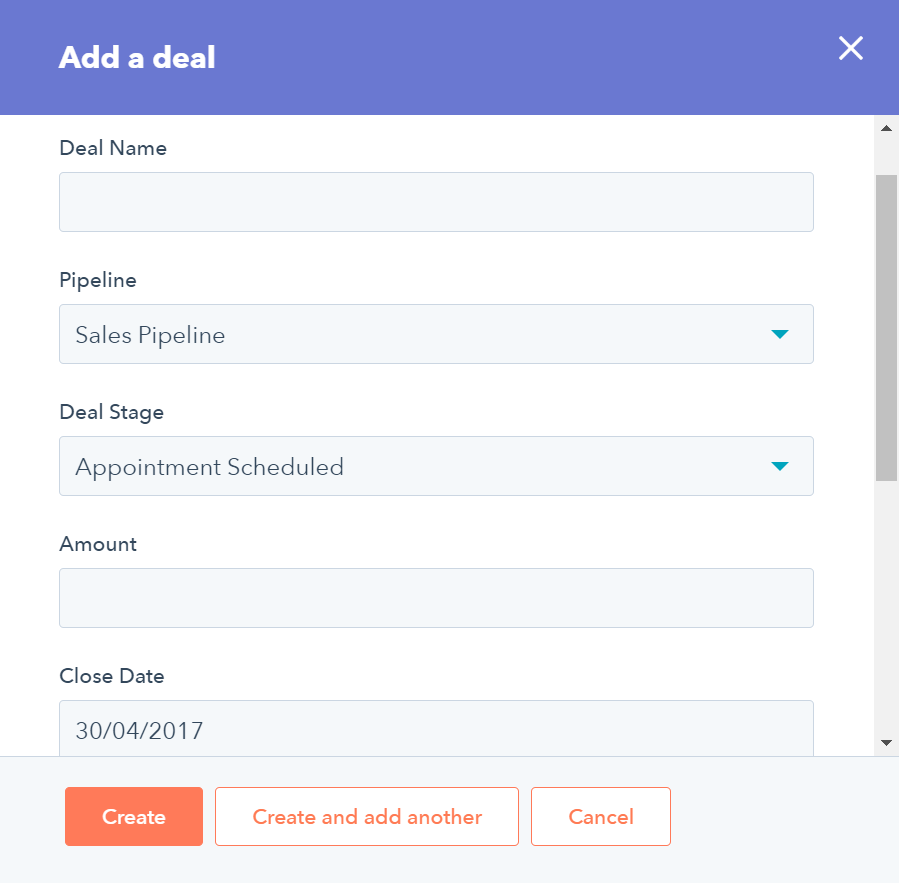
\includegraphics[width=0.5\textwidth]{deal_creation.png}
			\caption{Creando un deal desde el portal de HubSpot}
		\end{figure}

\subsection{company}
		
		Es un objeto de HubSpot que representa una empresa. Este objeto cuenta con multitud de propiedades, que describen información de la empres, como puede ser información de contacto, localización \ldots 
		
		Desde el portal de HubSpot es posible tanto crear nuevas companies como modificar cualquiera de los ya existentes.
		
		\begin{figure}
			\centering
			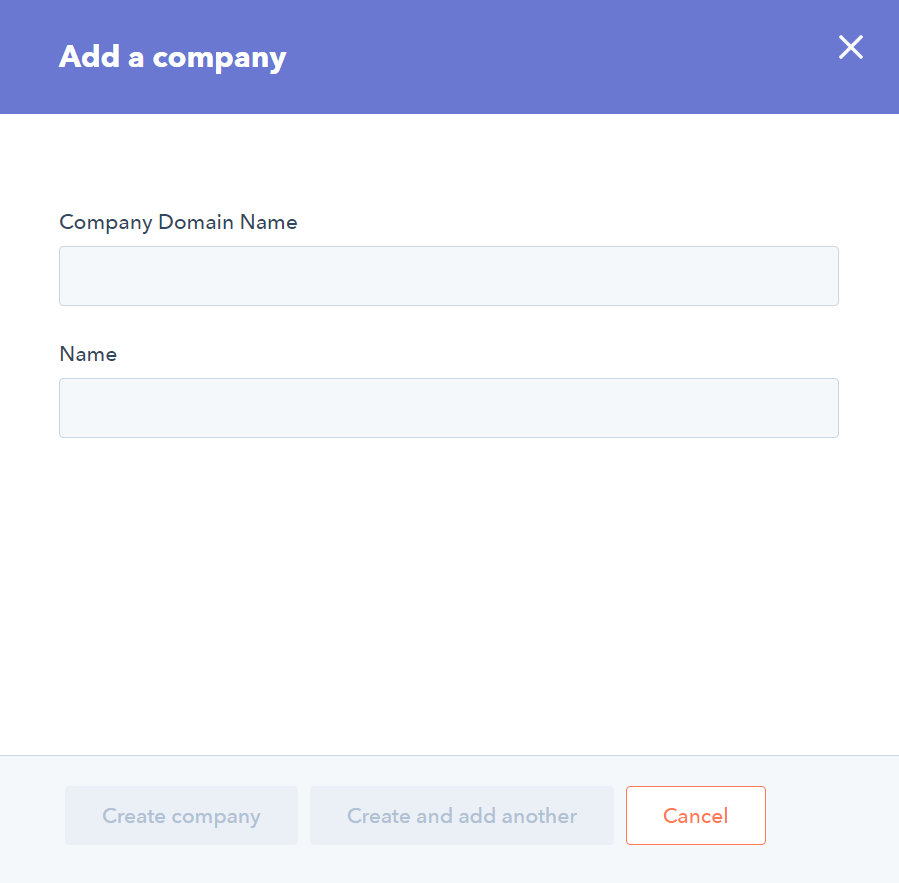
\includegraphics[width=0.5\textwidth]{company_creation.png}
			\caption{Creando una company desde el portal de HubSpot}
		\end{figure}


\subsection{Aplicación de Hubspot}
\label{subsec:app_hs}
%TODO API to glossary
Para poder realizar la integración y hacer uso de la API de HubSpot, es necesario crearse una cuenta de desarrollador. Con la cuenta de desarrollador podemos crear una aplicación y acceder a su panel de control. 
Desde el panel de control de la aplicación tendremos acceso a información importante para la integración, como son las claves (\verb|Client ID|, \verb|Client secret|).


También desde el panel de control de la aplicación deberemos especificar debemos indicar la dirección a la que deseamos que nuestros mensajes sean enviados y especificar los eventos de HubSpot ante los que se debe enviar un mensaje
En el caso de nuestra aplicación está suscrita a los siguientes eventos:

\begin{itemize}
	\item \textbf{deal.creation}: Cuando un nuevo deal es creado en HubSpot se envía un mensaje.
	\item \textbf{deal.propertyChanged} 
		\begin{itemize}
			\item \verb|dealstage|: Cuando en un deal de HubSpot se modifica el estado.
			\item \verb|practice|: Cuando en un deal de HubSpot se modifica la práctica.
			\item \verb|hubspot_owner_id|: Cuando en un deal de HubSpot se modifica su propietario.
			\item \verb|closedate|: Cuando en un deal de HubSpot se modifica la fecha de cierre.
			\item \verb|description|: Cuando en un deal de Hubspot se modifica la descripción.
			\item \verb|dealname|: Cuando en un deal de Hubspot se modifica el nombre.
			\item \verb|transaction_currency|: Cuando en un deal de HubSpot se modifica la moneda.
			\item \verb|legal_entity|: Cuando en un deal de HubSpot se modifica la entidad.
		\end{itemize}
\end{itemize}

Desde el panel de control de la aplicación de HubSpot también tenemos acceso a las claves (\verb|Client ID|, \verb|Client secret|) para poder instalar la aplicación en tantos portales como deseemos. En nuestro caso solo será uno.


Para instalar una aplicación en un portal de HubSpot hay que seguir un proceso de autorización llamado \gls{oauth2} que ha sido automatizado he integrado en la interfaz creada. 
Los pasos que hay que seguir son los siguientes \cite{hsapi}:
%TODO diagram oauth2

\begin{enumerate}
	\item Dirigirse a la url \url{https://app.hubspot.com/oauth/authorize?client_id=<client_id>&scope=contacts&redirect_uri=https://www.hubspot.com/}
		\\ 
		sustituyendo \textless client\_id\textgreater por el su valor. Y autorizar la instalación de la aplicación. Cabe destacar que solo se puede acceder a dicha url  y por tanto instalar la aplicación si se cuenta con el \verb|Client ID|.
		Haciendo público el \verb|Client ID| de la aplicación , esta puede ser instalada por cualquier persona. En nuestro caso este valor permanecerá en privado y solo nosotros haremos uso de la aplicación.
		
	\item Tras dar acceso al portal se te redirige a una página en la que aparece un código concatenado a la url.
	\item Mediante este código, el \verb|Client ID| y el \verb|Client secret| podemos obtener un token de sesión.
	Tras hacer la petición a la API de HubSpot, nos devolvera un mensaje con los siguientes valores.
		\begin{itemize}
			\item \verb|access_token| clave usado para realizar las peticiones a la API de HubSpot.
			\item \verb|refresh_token| usado para conseguir nuevo par (\verb|access_token|, \verb|refresh_token|) cuando el \verb|access_token| ha expirado.
			\item \verb|expires_in| tiempo en milisegundos de validez del \verb|access_token|.
		\end{itemize}
	\item Cuando el \verb|access_token| haya expirado podremos llamar a otro endpoint especificando el \verb|refresh_token| y recibiremos un mensaje de vuelta con otro nuevo \verb|access_token| y \verb|refresh_token|.
\end{enumerate}



\section{Interfaz}


Para el desarrollo de la Interfaz he usado el lenguaje de programación \textbf{python}, con el IDE \textbf{PyCharm}. La librería principal, bajo la que se sustenta el servidor es \textbf{web.py}.
Alternativas a esta librería pueden ser Flask o Django. Sin embargo esta última es para proyectos mucho más grandes. La ventaja de web.py es lo ligera qué es y la facilidad de ponerla en marcha.

La interfaz se encuentra ejcutandose de manera continua en un servidor y está escuchando en un puerto los distintos mensajes que puedan llegar de hubspot.
(En el panel de control de la aplicación de HubSpot ,explicado en la sección ~\ref{subsec:app_hs}, debemos especificar el host y puerto del servidor que está ejecutando la Interfaz)


\subsection{Estructura de la Interfaz}
Vamos a describir como se encuentra estructurada nuestra interfaz. Para ello podemos ver la figura ~\ref{fig:project_structure}. 

El proyecto de python se encuentra organizado en diferentes subdirectorios.

\begin{itemize}

	\item [\textendash] \textbf{service.py}: Se encuntra en el directorio raíz y se encarga de ejecutar la aplicación 
	y en este modulo está definida la función que se ejecuta al recibir un mensaje POST. Desde este módulo se hacen llamadas a distintas funciones de \textit{handler.py}.
	\item [\textendash] \textbf{handler.py}: También se encuentra en el directorio raíz y en este módulo se encuentra la lógica de programa para cada evento recibido.
	\item[$\square$] \textbf{hubspot}: En este directorio se encuentran todos los módulos de python que implementan funcionalidades para interactuar con HubSpot.
	
		\begin{itemize}
			\item [\textendash] \textbf{deal.py}: En este módulo se encuentra la clase Deal, encargada de representar en la Interfaz el objeto deal de HubSpot.
			\item [\textendash] \textbf{company.py}: En este módulo se encuentra la clase Company, que se encarga de representar al objeto company de HubSpot en la interfaz.
			\item [\textendash] \textbf{authorization.py}: En este módulo se encuentra la clase Authorization encargadada de facilitar el flujo de aprobación \gls{oauth2} de Hubspot y la renovación de los token de sesión.
		\end{itemize}
		
	\item[$\square$] \textbf{workday}: En este drectorio estan los módulos encargados de la interactuaión con Workday.
	
		\begin{itemize}
			\item [\textendash] \textbf{project.py}:
			\item [\textendash] \textbf{custommer.py}:
			\item [\textendash] \textbf{hierarchy.py}: 
		\end{itemize}
	\item[$\square$] \textbf{modules}: En este directorio se encuentran agrupados módulos con funcinalidades diversas. 
	
			\begin{itemize}
				\item [\textendash] \textbf{configuration.py}: 
				\item [\textendash] \textbf{database.py}:
				\item [\textendash] \textbf{log.py}:
				\item [\textendash] \textbf{mail.py}:
			\end{itemize}
			
	\item[$\square$] \textbf{cfg}: En este directorio se encuentran todos los archivos de configuración. 
	Por lo general permanecen invariantes. A excepción de aquellos que almacenan tokens de sesión que van cambiando.
	\item[$\square$] \textbf{xslt}: En este directorio se encuentran todas las plantillas de transformación necesarias para enviar los mensajes a Workday.
	Partiendo de un archivo xml, podemos transformarlo con estas plantillas y generar un mensaje SOAP para su posterior envío a Workday.
	

\end{itemize}

\begin{figure}
\centering
\tikzstyle{every node}=[draw=black,thick,anchor=west]
\tikzstyle{python}=[draw=blue,very thick, fill=blue!10, rounded corners]
\tikzstyle{folder}=[draw=orange,very thick,fill=orange!10]
%\tikzstyle{cfg}=[draw=red,fill=gray!50]
%\tikzstyle{xslt}=[draw=red,fill=gray!50]
\begin{tikzpicture}[
	scale=0.9,
  grow via three points={one child at (0.5,-1) and
  two children at (0.5,-1) and (0.5,-2)},
  edge from parent path={(\tikzparentnode.south) |- (\tikzchildnode.west)}]
	
	\node [folder]{ \Large Interfaz}
    child { node [python]{service.py}}		
    child { node [python]{handler.py}}
    child { node [folder] {hubspot}
      child { node [python]{deal.py}}
      child { node [python]{company.py}}
      child { node [python]{authorization.py}}
    }
	child [missing] {}				
    child [missing] {}				
    child [missing] {}
	child { node [folder] {workday}
      child { node [python]{project.py}}
      child { node [python]{customer.py}}
      child { node [python]{hierarchy.py}}
    }
	child [missing] {}				
    child [missing] {}				
    child [missing] {}
	child { node [folder] {modules}
      child { node [python]{configuration.py}}
      child { node [python]{database.py}}
      child { node [python]{log.py}}
	  child { node [python]{mail.py}}
    }
	child [missing] {}				
    child [missing] {}				
    child [missing] {}
	child [missing] {}				
	child { node [folder] {cfg}}
	child { node [folder] {xslt}};
	
	
	
\end{tikzpicture}
\caption{Estructura de la interfaz} \label{fig:project_structure}
\end{figure}

%TODO ver cada carpeta




\subsection{Almacenamiento persistente}

En nuestra intrfaz existen dos tipos de almacenamiento persistente. 

\begin{itemize}[leftmargin=*]
\item El primero de ellos ese trata de los archivos de configuración que se pueden ver en la figura ~\ref{fig:cfg_structure}.
En estos archivos se guarda información como usuarios, contraseñas, token de sesión, direcciones url. 
De esta forma se evita que estos datos este \textit{Hardcodeados} en el código, nos fácilita su modificación e
incluso la posibilidad de excluirlos facilmente cuando se añada el proyecto a repositorios públicos.
Para su impementación he usado la librería ConfigParser \cite{ConfigParser}.


\begin{figure}
\centering
\tikzstyle{every node}=[draw=black,thick,anchor=west]
\tikzstyle{python}=[draw=blue,very thick, fill=blue!10, rounded corners]
\tikzstyle{folder}=[draw=orange,very thick,fill=orange!10]
\tikzstyle{cfg}=[draw=red,fill=red!5]
%\tikzstyle{xslt}=[draw=red,fill=gray!50]
\begin{tikzpicture}[
	scale=0.9,
  grow via three points={one child at (0.5,-1) and
  two children at (0.5,-1) and (0.5,-2)},
  edge from parent path={(\tikzparentnode.south) |- (\tikzchildnode.west)}]
	
	\node [folder]{ \Large cfg}
    child { node [cfg]{hubspot.ini}}
    child { node [cfg]{workday.ini}}
    child { node [cfg]{mapping.ini}}
	child { node [cfg]{mail.ini}};
	
	
	
\end{tikzpicture}
\caption{Estructura de los archivos de configuración} \label{fig:cfg_structure}
\end{figure}


\item Por otro lado esta la base de datos local SQLite3 \cite{sqlite3} para python.
 En esta base de datos se almacena la correspondencia entre los deals de HubSpot y los proyectos de Workday.
 
 Exiten tres tablas en la base de datos: \verb|deals_excluded|, \verb|deal_project| y \verb|company_customer|.
 
 
 \begin{itemize}
	\item \verb|deals_excluded|: En esta tabla se almacena los identificadores de los deals de HubSpot 
	que se encuentran excluidos para la integración. Todos los deals que se encuentren en la fase de
	cierre estarán excluidos.
	\item \verb|deal_project|: En esta tabla se encuntran la correspondencias entre identificadores 
	de deals de HubSpot y los identificadores de los proyectos en Workday para todos los deals que han sido integrados.
	\item \verb|company_customer|: En esta tabla se encuntra la correspondencia entre las company de HubSpot y los clientes de Workday
	para todos los clientes que hayan sido integrados.
 \end{itemize}
 
\begin{table}
		\centering
		\begin{tabular}{
		|c|c@{\hskip 1cm} 
		|c|c|c@{\hskip 1cm} 
		|c|c|c@{\hskip 1cm}
		}
		\cline{1-1}\cline{3-4}\cline{6-7}
		deals\_excluded && \multicolumn{2}{c|}{deals\_excluded} && \multicolumn{2}{c|}{company\_customer} \\
	\cline{1-1}\cline{3-4}\cline{6-7}
	deal id && deal id & project id && company id & customer id \\
	\cline{1-1}\cline{3-4}\cline{6-7}
	\end{tabular}
	\caption{Tablas en la base de datos local}
	\label{tab:tables}
\end{table}

\end{itemize}




\subsection{Seguridad}


La interfaz se encuentra escuchando los mensajes que le son enviados. Pero ¿Cómo podemos garantizar que el mensaje que recibimos proviene realmente de HubSpot?
Para ello existe un campo en la cabecera del mensaje recibido, que es \verb|HUBSPOT_SIGNATURE|. 
Este campo es el formado tras aplicar la función hash \textbf{sha256} a la concatenación del \verb|Client Secret| de nuestra aplicación de HubSpot con el cuerpo del mensaje HTTP recibido.

Basta hacer esta comprobación para garantizar la procedencia del mensaje, ya que el \verb|Client Secret| solo es conocido por nosotros y por HubSpot. 
Además cabe destacar que cualquier persona que interceptase el mensaje, no podría deducir el \verb|Client Secret|, gracias a las propiedades de las funciones hash. %TODO cite function hash


Como podemos comprobar en la figura ~\ref{fig:validation_message}, aquellos mensajes que no cumplen los requisitos, se ignoran.

\begin{figure}
\centering

\shorthandoff{'}



\tikzstyle{line} = [draw, -latex']
\tikzstyle{startstop} = [rectangle, rounded corners, minimum width=3cm, minimum height=1cm,text centered, draw=black, fill=red!30]
\tikzstyle{io} = [trapezium, trapezium left angle=70, trapezium right angle=110, minimum width=3cm, minimum height=1cm, text centered, draw=black, fill=blue!30]
\tikzstyle{process} = [rectangle, minimum width=3cm, minimum height=1cm, text centered, draw=black, fill=orange!30]
\tikzstyle{decision} = [diamond, aspect=2,  minimum width=3cm, minimum height=1cm, text centered, draw=black, fill=green!30]
    
\begin{tikzpicture}[node distance = 3cm, auto]
	
	\node [io] (message) {Mensaje externo};
	\node [decision,below of =message] (valid) {¿Válido?};
	\node [startstop, below right of=valid, xshift=2cm, yshift=1cm] (no_valid) {Se ignora};
	\node [decision,below of =valid] (tipo) {¿Tipo?};
	
	\node [process, below left of=tipo, xshift=-2cm] (deal_creation) {Crear deal};
	\node [process, below right of=tipo, xshift=2cm] (deal_modification) {Modificar deal};
	
	\path [line] (message) -- (valid);
	\path [line] (valid.east) -| node {no}(no_valid);
	\path [line] (valid.south) -- node {sí}(tipo);
	
	\path [line] (tipo.west) -| node [left] {deal creation}(deal_creation);
	\path [line] (tipo.east) -| node {deal modfication}(deal_modification);
	
	
\end{tikzpicture}



\caption{Validación de los mensajes recibidos por la Interfaz} \label{fig:validation_message}
\end{figure}


\subsection{Flujo del programa}
%Dependiendo de de las acciones realizadas en HubSpot, se puede disparar un evento y que consiguientemente un mensaje se envíe a la interfaz.

Como se ha mencionado anteriormente, nuestra aplicación de HubSpot está suscrita a diferentes eventos de los deals de Hubspot.
Para explicar el flujo del programa, vamos a distinguir los eventos en dos tipos, creación de un deal y modificación de una propiedad de un deal.

\begin{itemize}
	\item \textbf{Creación de un deal}: Primero se recibe la petición \acrshort{http} por el método POST, que indica que un deal ha sido creado. En el cuerpo del mensaje se especifica el id del deal creado y otros datos de relevancia como el id del portal, id de la aplicación, momento en el que ocurrio el evento... \\
	
		Se comprueba si dicho deal se encuentra en la tabla \verb|deals_excluded| de base de datos local (Esta comprobación sirve como precaución para no crear proyectos no deseados en Workday).
		En caso de que este excluido, entonces la petición no se procesa.
		
		Si el deal no está excluido, se comprueba si existe una fila en la tabla de correspondecias \verb|deals_project| de la base de datos local.
		con la columna deal igual a la que se está procesando %(En la tabla \verb|deals_project| se guarda la correspondecia entre los identificadores
		%de los deals de HubSpot y los identificadores de los projectos de Workday que ya han sido integrados).
		En caso de que este en la tabla de correspondecias, entonces la petición se ignora.

		Si por el contrario no se encuentra en la tabla de correspondecias entonces se realiza una petición a HubSpot para obtener el resto de información del deal.
		Con todos los datos del deal que se ha creado se comprueba si se encuentra en la fase de progreso, en caso contrario dicho deal no se integra.
		
		
		
		Cada deal en HubSpot tiene asociado una \verb|copany| que se corresponde con un \verb|customer|
		Si el deal se encuentra en la fase de progreso, entonces se comprueba si la \verb|copany| asociada a este deal existe ya en workday, para ello se consulta la tabla de correspondencias \verb|company_customer|. Si no existe el correspondiente \verb|customer| en Workday, se crea.
		Después se crea el \verb|project| asociandolo con el previammente creado o existente \verb|customer|.
		
		
		\begin{figure}
\centering

\shorthandoff{'}



\tikzstyle{line} = [draw, -latex']
\tikzstyle{startstop} = [rectangle, rounded corners, minimum width=3cm, minimum height=1cm,text centered, draw=black, fill=red!30]
\tikzstyle{io} = [trapezium, trapezium left angle=70, trapezium right angle=110, minimum width=3cm, minimum height=1cm, text centered, draw=black, fill=blue!30]
\tikzstyle{process} = [rectangle, minimum width=3cm, minimum height=1cm, text centered, draw=black, fill=orange!30]
\tikzstyle{decision} = [diamond, aspect=2, minimum width=3cm, minimum height=1cm, text centered, draw=black, fill=green!30]
    
\begin{tikzpicture}[node distance = 3cm, auto]
	
	\node [startstop] (deal_creation) {Crear \textit{Deal}};
	\node [decision,below of =deal_creation] (db) {¿Está en BD?};
	\node [startstop, below right of=db, xshift=2cm, yshift=1cm] (in_db) {Se ignora el mensaje};
	\node [process,below of =db] (get_deal) {Obtener \textit{deal} de HubSpot};
	\node [decision,below of =get_deal] (valid) {\begin{tabular}{c}¿\textit{Dealstage} \\ válido? \end{tabular}};
	\node [process, below of=valid] (submit_customer) {Subir \textit{customer} a Workday};
	\node [process, below of=submit_customer] (submit_project) {Subir \textit{project} a Workday};
	
	
	\path [line] (deal_creation) -- (db);
	\path [line] (db.east) -| node {si}(in_db);
	\path [line] (db.south) -- node {no}(get_deal);
	\path [line] (get_deal.south) -- (valid);
	\path [line] (valid.south) -- node [left] {si} (submit_customer);
	\path [line] (valid.east) -| node [right] {no} (in_db);
	\path [line] (submit_customer.south) -- (submit_project);
	
	
\end{tikzpicture}



\caption{Proceso Crear Deal} \label{fig:deal_creation}
\end{figure}
		
		
	\item \textbf{Modificación de un deal}:
		Se comprueba si dicho deal se encuentra en la tabla \verb|deals_excluded| de base de datos local. En tal caso, no se sincronizan las modificaciones en Workday.
		En caso de que no sea excluido, se comprueba si existe en la tabla de correspondencias \verb|deal_project|. De no ser así se procede a la creación del deal detallada anteriormente.
		
		
		
		Se obtiene el objeto \verb|project| de Workday. Se actualizan los correspondientes campos localmente, dependiendo de la propiedad del deal que haya cambiado. Por último se actualiza el objeto \verb|project| correspondiente de Workday con los cambios realizados.
		
		%TODO diagram with the modification of a deal
		
		\begin{figure}[H]
\centering

\shorthandoff{'}



\tikzstyle{line} = [draw, -latex']
\tikzstyle{startstop} = [rectangle, rounded corners, minimum width=3cm, minimum height=1cm,text centered, draw=black, fill=red!30]
\tikzstyle{io} = [trapezium, trapezium left angle=70, trapezium right angle=110, minimum width=3cm, minimum height=1cm, text centered, draw=black, fill=blue!30]
\tikzstyle{process} = [rectangle, minimum width=3cm, minimum height=1cm, text centered, draw=black, fill=orange!30]
\tikzstyle{decision} = [diamond, aspect=2, minimum width=3cm, minimum height=1cm, text centered, draw=black, fill=green!30]
    
\begin{tikzpicture}[node distance = 3cm, auto]
	
	\node [startstop] (deal_modification) {Modificar Deal};
	\node [decision,below of =deal_modification] (db) {¿Está en BD?};
	\node [process, below right of=db, xshift=2cm, yshift=1cm] (not_in_db) {Crear Deal};
	\node [process,below of =db] (get_deal) {Obtener deal de HubSpot};
	\node [process, below of=get_deal] (update_project) {Subir project en Workday};
	
	
	\path [line] (deal_modification) -- (db);
	\path [line] (db.east) -| node {no}(not_in_db);
	\path [line] (db.south) -- node {si}(get_deal);
	\path [line] (get_deal.south) -- (update_project);
	
	
\end{tikzpicture}



\caption{Proceso Modificar Deal} \label{fig:deal_modification}
\end{figure}

\end{itemize}



